%%%%%%%%%%%%%%%%%%%%%%%%%%%%%%%%%%%%%%%%%
% Beamer Presentation
% LaTeX Template
% Version 1.0 (10/11/12)
%
% This template has been downloaded from:
% http://www.LaTeXTemplates.com
%
% License:
% CC BY-NC-SA 3.0 (http://creativecommons.org/licenses/by-nc-sa/3.0/)
%
%%%%%%%%%%%%%%%%%%%%%%%%%%%%%%%%%%%%%%%%%

%----------------------------------------------------------------------------------------
%	PACKAGES AND THEMES
%----------------------------------------------------------------------------------------

\documentclass{beamer}

\mode<presentation> {

% The Beamer class comes with a number of default slide themes
% which change the colors and layouts of slides. Below this is a list
% of all the themes, uncomment each in turn to see what they look like.

%\usetheme{default}
%\usetheme{AnnArbor}
%\usetheme{Antibes}
%\usetheme{Bergen}
%\usetheme{Berkeley}
%\usetheme{Berlin}
%\usetheme{Boadilla}
%\usetheme{CambridgeUS}
%\usetheme{Copenhagen}
%\usetheme{Darmstadt}
%\usetheme{Dresden}
%\usetheme{Frankfurt}
%\usetheme{Goettingen}
%\usetheme{Hannover}
%\usetheme{Ilmenau}
%\usetheme{JuanLesPins}
%\usetheme{Luebeck}
\usetheme{Madrid}
%\usetheme{Malmoe}
%\usetheme{Marburg}
%\usetheme{Montpellier}
%\usetheme{PaloAlto}
%\usetheme{Pittsburgh}
%\usetheme{Rochester}
%\usetheme{Singapore}
%\usetheme{Szeged}
%\usetheme{Warsaw}

% As well as themes, the Beamer class has a number of color themes
% for any slide theme. Uncomment each of these in turn to see how it
% changes the colors of your current slide theme.

%\usecolortheme{albatross}
%\usecolortheme{beaver}
%\usecolortheme{beetle}
%\usecolortheme{crane}
%\usecolortheme{dolphin}
%\usecolortheme{dove}
%\usecolortheme{fly}
%\usecolortheme{lily}
%\usecolortheme{orchid}
%\usecolortheme{rose}
%\usecolortheme{seagull}
%\usecolortheme{seahorse}
%\usecolortheme{whale}
%\usecolortheme{wolverine}

%\setbeamertemplate{footline} % To remove the footer line in all slides uncomment this line
%\setbeamertemplate{footline}[page number] % To replace the footer line in all slides with a simple slide count uncomment this line

%\setbeamertemplate{navigation symbols}{} % To remove the navigation symbols from the bottom of all slides uncomment this line
}

\usepackage{graphicx} % Allows including images
\usepackage{booktabs} % Allows the use of \toprule, \midrule and \bottomrule in tables
\usepackage{listings}
\usepackage{amsmath}
\usepackage{algpseudocode,algorithm,algorithmicx}

\lstdefinestyle{customjava}{
  breaklines=true,
  frame=L,
  xleftmargin=\parindent,
  language=Java,
  showstringspaces=false,
  basicstyle=\footnotesize\ttfamily,
  keywordstyle=\bfseries\color{green!40!black},
  commentstyle=\itshape\color{gray!40!black},
  identifierstyle=\color{blue},
  stringstyle=\color{orange},
}

\lstdefinestyle{customcpp}{
  breaklines=true,
  frame=L,
  xleftmargin=\parindent,
  language=C++,
  showstringspaces=false,
  basicstyle=\footnotesize\ttfamily,
  keywordstyle=\bfseries\color{green!40!black},
  commentstyle=\itshape\color{gray!40!black},
  identifierstyle=\color{blue},
  stringstyle=\color{orange},
}
%----------------------------------------------------------------------------------------
%	TITLE PAGE
%----------------------------------------------------------------------------------------

\title[Processes 2]{Processes 2} % The short title appears at the bottom of every slide, the full title is only on the title page

\author{Jonathan Windle} % Your name
\institute[UEA] % Your institution as it will appear on the bottom of every slide, may be shorthand to save space
{
University of East Anglia \\ % Your institution for the title page
\medskip
\textit{J.Windle@uea.ac.uk} % Your email address
}
\date{\today} % Date, can be changed to a custom date

\begin{document}

\begin{frame}
\titlepage % Print the title page as the first slide
\end{frame}

\begin{frame}[allowframebreaks]
\frametitle{Overview} % Table of contents slide, comment this block out to remove it
\tableofcontents % Throughout your presentation, if you choose to use \section{} and \subsection{} commands, these will automatically be printed on this slide as an overview of your presentation
\end{frame}

%-------------------------------------------------------------------
\section{Types of Process}
\begin{frame}
\frametitle{Types of Process}
\begin{itemize}
\item Compute bound:\\
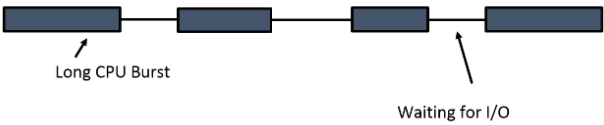
\includegraphics[scale=0.3]{compute.png}
\item I/O bound:\\
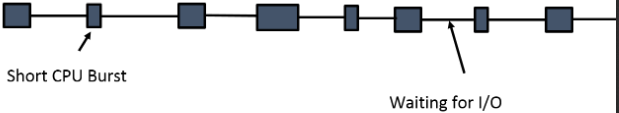
\includegraphics[scale=0.3]{io.png}\\
\item Types of Scheduling Algorithm:
\begin{itemize}
\item Nonpreemptive
\begin{itemize}
\item Picks a process to run and lets it run until it blocks or completes.
\end{itemize}
\item Preemptive:
\begin{itemize}
\item Picks a process to run and lets it run for a fixed period of time.
\end{itemize}
\end{itemize}
\end{itemize}
\end{frame}
%------------------------------------------------------------------
\section{When to schedule}
\begin{frame}
\frametitle{When to Schedule}
\begin{enumerate}
\item When a process switches from the running state to the waiting state.
\begin{itemize}
\item e.g. When it blocks waiting for I/O
\end{itemize}
\item When a process switches from the running state to the ready state.
\begin{itemize}
\item e.g. When an interrupt occurs
\end{itemize}
\item When a process switches from the waiting state to the ready state.
\begin{itemize}
\item e.g. When an I/O operation completes.
\end{itemize}
\item When a process terminates
\end{enumerate}
Nonpreemptive scheduling takes place under circumstances 1 and 4 only. Others are preemptive.
\end{frame}
%-------------------------------------------------------------------
\section{Scheduling Goals}
\begin{frame}
\frametitle{Scheduling Goals}
\begin{itemize}
\item All scheduling algorithms should be fair.
\item Scheduling policies must be enforced.
\begin{itemize}
\item Safety controll processes should get priority (even if the payroll is delayed).
\end{itemize}
\item All parts of the system should be kept busy )as this gets more work done per second than if some are idle).
\begin{itemize}
\item In a batch system, where the scheduler controls which jobs are brought into memory, its better to have a mix of CPU bound and I/O bound processes.
\end{itemize}
\end{itemize}
\end{frame}
%------------------------------------------------------------------
\section{Computing Environments}
\begin{frame}
\frametitle{Computing Environments}
\begin{itemize}
\item Batch:
\begin{itemize}
\item No user interaction, processes can be switched infrequently.
\item Aim to maximize throughput and CPU utilization.
\item Nonpreemptive scheduling is used.
\end{itemize}
\item Interactive
\begin{itemize}
\item Processes must reflect user actions e.g. Time-shared multiprogramming
\item Aim to minimize responsee time
\item Preemptive scheduling is needed
\end{itemize}
\item Real-Time
\begin{itemize}
\item System must meet real-time constraints
\item Well designed systems to not need preemptive scheduling.
\end{itemize}
\end{itemize}
\end{frame}
%-----------------------------------------------------------------
\section{Scheduling Algorithms}
\begin{frame}
\frametitle{Scheduling Algorithms}
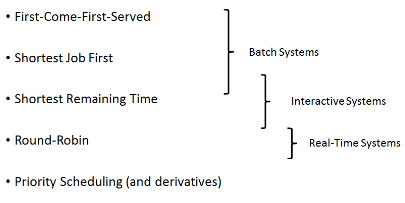
\includegraphics[scale=0.5]{specif.png}
\end{frame}
%-------------------------------------------------------------------
\subsection{First-Come-First-Serve}
\begin{frame}
\frametitle{First-Come-First-Serve}
\begin{itemize}
\item The process that has waited longest, goes next.
\item Process then run to completion or blocked (nonpreemptive)
\item Advantages:
\begin{itemize}
\item Queue does not need to be ordered
\item Simple
\item Fair
\end{itemize}
\item Disadvantages:
\begin{itemize}
\item No consideration on throughput
\item Potentially long turnaround (if the queue is large).
\item Short or I/O bound processes are penalised.
\end{itemize}
\end{itemize}
\end{frame}
%-------------------------------------------------------------------
\subsection{Shortest Job First}
\begin{frame}
\frametitle{Shortest Job First}
\begin{itemize}
\item Ordered by time to complete 
\item Allowed to run until complete (nonpreemptive)
\item Reordered at context switch
\item Allows high throughput but penalises long processes.
\item Open to abuse - hard to accurately estimate required time.
\item Processes could underestimate the required time to jump ahead in the queue.
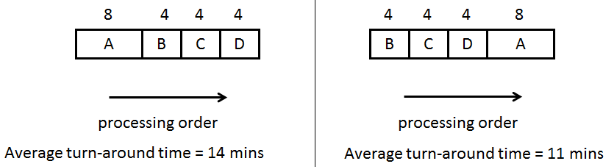
\includegraphics[scale=0.35]{short.png}
\end{itemize}
\end{frame}
%----------------------------------------------------------------
\subsection{Shortest time Remaining}
\begin{frame}
\frametitle{Shortest time Remaining}
\begin{itemize}
\item Order processed by closest time to completion.
\item As new jobs are submitted, choose the job closest to terminating.
\item Provides good throughput and response time
\item Still penalises long processes.
\item Difficult to predict remaining time.
\item Advantages:
\begin{itemize}
\item Favours new ``short" processes.
\item Optimises throughput
\end{itemize}
\item Disadvantages:
\begin{itemize}
\item Penalises long processes.
\end{itemize}
\end{itemize}
\end{frame}
%------------------------------------------------------------------
\subsection{Round Robin}
\begin{frame}
\frametitle{Round Robin}
\begin{itemize}
\item Defines unit of time (typically 10-50ms) called the {\color{red}quantum}
\item If it's too short, the system ends up context switching a lot, if it's too long, the system is sluggish and unresponsive.
\item Selective process runs for the {\color{red}quantum} amount of time.
\item After the {\color{red}quantum} expires, the CPU is relinquished and process moved to the back of the queue.
\item Process at the front is then allocated the CPU for a quantum.
\item Advantages:
\begin{itemize}
\item Fair
\item Easy to implement
\end{itemize}
\item Disadvantages:
\begin{itemize}
\item I/O bound processes are penalised.
\item Length of quantum must be carefully chosen to achieve maximum throughput.
\item No account of priority.
\end{itemize}
\end{itemize}
\end{frame}
%-------------------------------------------------------------------
\subsection{Priority Scheduling}
\begin{frame}
\frametitle{Priority Scheduling}
\begin{itemize}
\item Each process is assigned a priority, so after the quantum expires, the process with the next highest priority is selected.
\item Static priority: Priority is fixed for the lifetime of the process.
\item Dynamic priority: 
\begin{itemize}
\item Priority varies on the CPU usage pattern.
\item Multiply priority by 100/x for the next schedule, where x is \% of quantum used.
\item Fairer for I/O bound processes that do not utilise the CPU much before blocking.
\end{itemize}
\item Advantages:
\begin{itemize}
\item Simple to implement, fair
\end{itemize}
\item Disadvantages:
\begin{itemize}
\item Can suffer priority inversion if static.
\end{itemize}
\end{itemize}
\end{frame}
%--------------------------------------------------------------------
\subsection{Multiple Queue Schedular}
\begin{frame}
\frametitle{Multiple Queue Schedular}
\begin{itemize}
\item Groups processes into priority classes:
\begin{itemize}
\item Uses priority scheduling among the classes.
\item Uses round-robin scheduling withing each class.
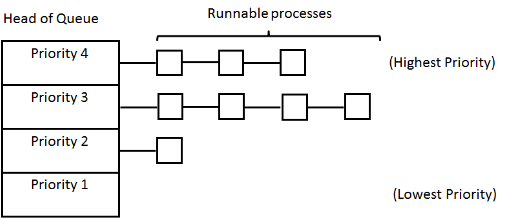
\includegraphics[scale=0.3]{mult.png}
\end{itemize}
\end{itemize}
\end{frame}
%---------------------------------------------------------------------
\subsection{Lottery Scheduling}
\begin{frame}
\frametitle{Lottery Scheduling}
\begin{itemize}
\item Give each process a lottery ticket for resources (e.g. CPU time).
\item At next context switch, the schedular draws a ticket at random, process holding ticket gets the resource.
\item Higher priority processes are given more tickets and therefore higher chance of being chosen.
\item New processes have a chance of winning immediately so the system appears responsive.
\item Tickets can be exchanged between processes to temporarily increase the priority.
\item Advantages:
\begin{itemize}
\item Allocation of tickets reflects fraction of resources allocated.
\item Chance of winning is always determined by number of tickets held.
\item Cooperating processes can exchange tickets if they wish.
\end{itemize}
\end{itemize}
\end{frame}
%-----------------------------------------------------------------
\section{Summary}
\begin{frame}
\frametitle{Summary}
\begin{itemize}
\item To hide the effects of interrupts (difficult and dangerous for users to manage) operating systems provide  conceptual model consisting of sequentil processes.
\item Two classes of process:
\begin{itemize}
\item Compute bound
\item I/O bound
\end{itemize}
\item Two classes of schedular:
\begin{itemize}
\item Nonpreemptive
\item preemptive.
\end{itemize}
\item Different scheduling algorithms have different properties and a choice of particular algorithm may favour one class of process over another.
\end{itemize}
\end{frame}
%------------------------------------------------------------------

\begin{frame} 
\Huge{\centerline{The End}}
\end{frame}

\end{document}